\chapter{Defeasible Reasoning}
\label{chapter:defeasible-reasoning}

Non-monotonicity in logical systems has been the focus of study for decades, and several distinct formalisms have been developed.
The motivation is to expand the inference power beyond that of the classical, to a more credulous one where inferences may,
upon learning new information, be retracted.

This work is interested in the kind of non-monotonic reasoning put forward by Kraus, Lehmann, and Magidor \cite{kraus1990nonmonotonic,lehmann1992what},
frequently initialised to the \textit{KLM framework}.

\textcolor{red}{This could be a bit more discursive I think}

\section{Background on Non-monotonic Reasoning}
\label{section:nmr-background}

Near the end of the previous chapter, the matter of consequence was discussed in a very formal sense. It is perhaps
helpful to distinguish this subject---classical consequence---from the common concept, as the former yields some surprising
results which do not appear at all congruent with how a person, or otherwise intelligent agent should reason
\cite{tarski1936consequence,kraus1990nonmonotonic}. As a demonstration of a result which may be surprising in this way,
consider the following propositions, which state that \textit{humans experience chronological time \text{,} soldiers are
	human}, and \textit{Billy Pilgrim experiences non-chronological time}.
\begin{enumerate}
	\item $\texttt{human}\rightarrow \texttt{chronological time}$

	\item $\texttt{soldier}\rightarrow \texttt{human}$

	\item $\texttt{Billy Pilgrim}\rightarrow \neg \texttt{chronological time}$
\end{enumerate}

Knowing these propositions, if we were to encounter an individual in combat fatigues we might find it sensible---by propositions
2 and 1---to deduce that the individual experienced time chronologically. If we were to later learn that the individual
were, in fact, Billy Pilgrim, given proposition 3, we should like to retract our prior inference and replace it with the
knowledge that the individual does not experience time chronologically.

Such recourse is not, as it stands, possible. When we see the that the individual is a soldier, the possible worlds
satisfying our existing knowledge are reduced to the single model: $\{\overline{b},c, h,s\}$ (where $b$: \texttt{Billy
	Pilgrim}, $c$: \texttt{chronological time}, $h$: \texttt{human}, and $s$: \texttt{soldier}). Should we later learn that the
individual is indeed Billy Pilgrim, the theory becomes inconsistent.
%TODO: Add section in preliminaries about principle of explosion
And, by the principle of explosion, discussed in \Cref{subsection:logical-consequence}, our theory now entails that the
individual experiences time both chronologically and non-chronologically. Indeed, our theory now entails everything and
is accordingly worthless.

This property of classical logic---that adding new information never results in retraction of pre-existing knowledge---is
called monotonicity. The presence of monotonicity requires that when we make a claim such as \say{humans experience time chronologically},
we must be absolutely sure of ourselves, so as to never worry about needing to retract an inference. This is, of course,
too strict a requirement as we cannot determine for all future, present, and past humans if it were the case that they experienced
time chronologically. If we remain in the classical realm, it seems our only options are to abandon our original claim or
risk explosion.

At this point it is a good idea to provide some clarification on how we might begin to approach solutions to this issue.
Continuing with the same example---and continuing to allow ourselves to entertain the possibility of experiencing non-chronological
time---it would certainly be agreed that typically soldiers are human, and also that typically humans experience time chronologically.
To resolve that Billy Pilgrim is a soldier, and therefore a human, who does not experience chronological time, we need only
to point out that he may be an atypical human, and so the qualities we associate with typical humans need not apply to
him.

To make the previous paragraph more formal, we remind the reader of the discussion held around \Cref{definition:logical-consequence}:
A formula $\phi$ is a logical consequence of a set $\Gamma$ thereof if every model of $\Gamma$ is also a model of $\phi$.
Put differently, there is no valuation (or, possible world) where $\Gamma$ is true and $\phi$ is false. It follows
directly that $\phi$ remains a logical consequence of $\Gamma \cup \{\psi\}$, since $\Gamma$ is true in any world where $\Gamma
	\cup \{\psi\}$ is true. It was pointed out in \cite{shohamSemanticApproach} that we may \say{bend the rules} and restrict
semantic consideration to a privileged subset of models deemed ``preferable''. We call these selected models the \textit{minimal
	models}---the reasons for this name should become clearer as the chapter progresses.

\section{Preferential Reasoning and the KLM Framework}
\label{section:klm-framework}

The KLM framework for non-monotonic reasoning was initially described by a collection of consequence relations
satisfying certain axioms---frequently called the \textit{rationality postulates}, thought to describe a reasonable
account of non-monotonic consequence. We borrow a nice story from \cite{gabbay1985theoreticalFoundations}, in which he
motivates why consequence relations are a good starting point for the study of non-monotonic systems.

Paraphrasing, he begins by asking the reader to imagine a machine that does non-monotonic inference in some domain. The
machine represents knowledge as formulae and so we pose queries of the form \say{Does $\psi$ non-monotonically follow from $\phi$?}.
Something goes awry (suppose some coffee was spilled), calling into question whether the logic of the machine still functions
correctly. Even worse, the interface, which tells us what real-world instance each formula maps to, is destroyed and so function
cannot be evaluated based on the meaning of the formulae the machine reasons on. How might we then evaluate the machine's
function?

If we were interested in classical consequence, we would be well-equipped to assess the correctness of the machine by determining
if it satisfied reflexivity, monotonicity, and cut (we point to \Cref{definition:consequence-relations} as a reminder).
This is precisely the starting point that Kraus, Lehmann, and Magidor took up in \shortcite{kraus1990nonmonotonic},
suggesting that before getting to the semantics of a non-monotonic system, it is a good idea to formalise axiomatise the
system as a consequence relation satisfying certain properties.

The rationality postulates are precisely this axiomatisation, characterising a sensible pattern of reasoning for non-monotonic
systems. We use `$\twiddle$' (pronounced ``twiddle'') instead of `$\vdash$' to denote a non-monotonic consequence relation.
As we may expect, $\phi \twiddle \psi$ has the same meaning as $(\phi, \psi) \in \; \twiddle$, and $\phi \ntwiddle \psi$
as $(\phi, \psi)\not \in \; \twiddle$. We may, at times of potential confusion, use a subscript to disambiguate which consequence
relation is being referred to, and so $\twiddle_{p}$ would refer to a cumulative relation, as defined below.

\subsection{System P}
\label{subsection:system-P} \index{non-monotonic reasoning! system P}

We will begin the exposition of the KLM framework by looking at \textit{system P}. The pattern of reasoning associated with
this system is captured by \textit{preferential consequence relations}. \textcolor{red}{Either we need to justify the
	choice of omitting cumulative relations, or include them.}

\begin{definition}
	\label{definition:preferential-relation}

	The consequence relation $\twiddle$ is a \emph{preferential consequence relation} if and only if it satisfies the properties
	of \emph{Reflexivity}, \emph{Left Logical Equivalence}, \emph{Right Weakening}, \emph{And}, \emph{Or}, and \emph{Cautious
		Monotony}.
\end{definition}
%
The first axiom, \textit{Reflexivity}, is largely self justifying. It makes little sense to speak about a notion of
consequence that does not satisfy this property.
%
\begin{align}
	\label{postulate:ref}\inferLeft{Reflexivity}{}{\phi \twiddle \phi}
\end{align}
%
The justification for \textit{Left Logical Equivalence} is a bit more opaque. The principle it describes is that if two scenarios
represent the same state of affairs, and in one of these scenarios it we typically expect some consequence, then we should
expect the same in the other scenario. \textcolor{red}{Invariant to substitution of logically equivalent formulas?}
%
\begin{align}
	\label{postulate:lle}\inferLeft{Left Logical Equivalence}{\vdash \phi \leftrightarrow \psi, \quad \phi \twiddle \gamma}{\psi \twiddle \gamma}
\end{align}
%
\textit{Right Weakening} allows the preservation of classical consequence within preferential logic. It says that, if
from $\phi$ we normally expect $\psi$, but from $\psi$ we \textit{always} see $\gamma$, then we are entitled to think that
from $\phi$ we normally expect $\gamma$ as well.
%
\begin{align}
	\label{postulate:rw}\inferLeft{Right Weakning}{\vdash \psi \rightarrow \gamma, \quad \phi \twiddle \psi}{\phi \twiddle \gamma}
\end{align}
%
As a justification for \textit{Or}, consider that \textit{Normally, if Billy were abducted by aliens he would be traumatised},
but also \textit{Normally, if Billy witnessed the fire-bombing of Dresden he would be traumatised}. If we learned that
either of these events took place, we should find it plausible to infer that Billy were traumatised.
%
\begin{align}
	\inferLeft{Or}{\phi \twiddle \gamma, \quad \psi \twiddle \gamma}{\phi \lor \psi \twiddle \gamma}
\end{align}
%
The \textit{And} postulate suggests that if $\psi$ and $\gamma$ are both expected consequence of $\phi$, then their
conjunction is also expected. This postulate fails in probabilistic systems, such as \textit{association rules} \cite{gabbay1985theoreticalFoundations}.
%
\begin{align}
	\label{postulate:and}\inferLeft{And}{\phi \twiddle \psi, \quad \phi \twiddle \gamma}{\phi \twiddle \psi \land \gamma}
\end{align}
%
\textit{Cautious Monotony} (which has also be called \textit{Cumulative Monotony} by \cite{makinson2003bridges}, and
\textit{Restricted Monotony} by \cite{gabbay1985theoreticalFoundations}) corresponds to the notion that if we are in an
epistemic state $\phi$ where one expectation, among others, is that $\psi$ holds. Learning that $\psi$ indeed holds should
not alter the epistemic state in such a way that the \textit{other} expectations are abandoned, and so the new state,
$\phi \land \psi$, we should expect everything that was expected when all we knew was $\phi$. In other words, we reason monotonically
with respect to expected information.
%
\begin{align}
	\label{postulate:cm}\inferLeft{Cautious Monotony}{\phi \twiddle \psi, \quad \phi \twiddle \gamma }{\phi \land \psi \twiddle \gamma}
\end{align}

The above postulates capture the essence of preferential (consequence) relations. Much like we saw with Hilbert systems,
however, certain rules, which reveal interesting properties of system P, may be derived. A version of \textit{Cut}:
%
\begin{align}
	\label{postulate:cut}\inferLeft{Cut}{\phi \land \psi \twiddle \gamma, \quad \phi \twiddle \psi}{\phi \twiddle \gamma}
\end{align}
%
The original version due to Gentzen \cite{Ben1993Mathematical}, which is presented as:
%
\begin{align}
	\inferLeft{Monotonic Cut}{\phi \land \psi \twiddle \gamma, \quad \alpha \twiddle \psi}{\phi \land \alpha \twiddle \gamma}
\end{align}
%
implies monotonicity, as it requires that if $\psi$ is a typical consequence of $\alpha$, then it must remain a consequence
of $\alpha \land \phi$: ergo, monotonicity. The former variation does not enforce this, and rather says \say{Suppose I have certain knowledge of $\phi$, and that if I were to assume $\psi$ I should expect to conclude $\gamma$. Then if I can show that infact $\psi$ was already an expected consequence of knowing $\phi$, I should expect that $\gamma$ follows from $\phi$}.
When considered alongside the argument for Cautious Monotony, Cut seems obviously acceptable.

The rule $S$, which is analogous to one half of the deduction theorem (cf. \Cref{axiom:deduction-theorem}), expresses the
notion that we retain plausible inferences when conditioned on a hypothesis.
%
\begin{align}
	\inferLeft{S}{\phi \land \psi \twiddle \gamma}{\phi \twiddle \psi \rightarrow \gamma}
\end{align}

The following Lemma is a helpful intuition pump: it suggests that we can use the consequences of plausible inferences to
make further plausible inferences.
%
\begin{lemma}
	\label{lemma:cut-cautious}

	We can cover the properties of \emph{cut} and \emph{cautious monotonicity} with the following principle: \say{If $\phi \twiddle \psi$, then the typical consequences of $\phi$ and $\phi \land \psi$ coincide}.
\end{lemma}

% \begin{align}
% 	\label{postulate:monotonicity}\inferLeft{Monotonicity}{\psi \rightarrow \gamma, \quad \gamma \twiddle \phi}{\psi \twiddle \phi}
% \end{align}
% %
% In addition, \textit{Transitivity} and \textit{Contraposition} both imply monotonicity when considered alongside the other
% rules of cumulative relations
% %
% \begin{align}
% 	\label{postulate:trans}\inferLeft{Transitivity}{\phi \twiddle \psi, \quad \psi \twiddle \gamma}{\phi \twiddle \gamma}
% \end{align}

% \begin{align}
% 	\label{postulate:contra}\inferLeft{Contraposition}{\phi \twiddle \psi}{\neg \psi \twiddle \neg \phi}
% \end{align}

% These properties are undesirable as they imply monotonicity.
It is, however, worth reminding ourselves of the goal that was set out at the start of this chapter: To formalise a system
which facilitates a more credulous style of reasoning. That is, we are interested in making \textit{more} inferences
than can be made under classical notions of consequence. One property which has not been discussed---and which may be quite
easy to assume---is whether the proposed system be \textit{supraclassical} \cite{makinson2003bridges}.
%
\begin{align}
	\label{postulate:supraclassical}\inferLeft{Supraclassical}{\phi \rightarrow \psi}{\phi \twiddle \psi}
\end{align}
%
Supraclassicality is the question of whether classical inferences be preserved in a non-classical system. It seems
reasonable to answer this question in the affirmative. Defeasible inferences are useful as they tolerate reasoning with exceptions,
allowing useful inferences that could not be made in classical systems. It seems that the dual of this, where some non-defeasible
(that is, classical) inference is made, it is because no exceptions apply. In this case, we have an even stronger claim
to make this inference.

\subsubsection{Preferential Interpretations}
\label{subsubsection:preferential-interpretations}

The semantics of system P, provided by Kraus, Lehmann, and Magidor \cite{kraus1990nonmonotonic}, are based on the \textit{preference
	logics} introduced by Shoham \cite{shohamSemanticApproach}. The fundamental idea is that valuations, or \textit{worlds},
can be ordered by a \textit{preference relation} so that one world being preferred to another is a normative claim that we
should consider deductions which hold in the preferred world---but may not in other worlds---as plausible.

It will be useful to recall some definitions from propositional logic: a valuation $u \in \mathcal{U}$ is a \textit{model}
of a formula $\phi \in \mathcal{L}$ if it satisfies $\phi$, $\phi$ is \textit{satisfiable} if it has a model. Another
formula $\psi$ is a \textit{logical consequence} of $\phi$ if the models of $\phi$ are a subset of the models of $\psi$.

We now introduce analogous definitions in the setting of preferential logic. The first change is that we consider a
richer language, $\Lang$, which is simply $\lang$ extended with the new connective `$\twiddle$' such that
$\phi \twiddle \psi$ is a sentence in $\Lang$ when $\phi, \psi \in \mathcal{L}$. It is easy to skip over, but usage of
the `$\twiddle$' has now shifted from an element of the metalanguage, where it refers to a kind of consequence relation,
to an object level connective, used analogously to the classical Boolean operator `$\rightarrow$'. Certain restrictions
on the usage of `$\twiddle$' do apply. In particular, the nesting of defeasible statements is not permitted, and so $\phi
	\twiddle (\psi \twiddle \gamma )$ is not a statement in the language $\Lang$. At times, we may wish to distinguish between
formulae in $\Lang$ which do not use `$\twiddle$', and so we refer to these as classical, and the alternative as defeasible
formulae.

\begin{definition}
	\label{definition:preferential-interpretation} \index{non-monotonic reasoning! system P! preferential interpretation}

	A \emph{preferential interpretation} $\Pin$ is a triple where $S$ is a set of \emph{states}, $l: S \to \mathcal{U}$ is
	a function mapping states to valuations, and $\prec$ is a strict partial-order on $S$.
\end{definition}

The preference relation provides a basis for restricting ourselves to consider only those preferred worlds, which represent
a normal state of affairs. This idea is formalised as \textit{minimal states}:

\begin{definition}
	\label{definition:state-minimal}

	Given a preferential interpretation $\Pin$ and some $\phi \in \Lang$, we write $\underline{\hat{\phi}}$ to denote the set
	$\{s \in \hat{\phi}\mid \nexists s' \in \hat{\phi}\text{ such that }s' \prec s \}$, which is the set of \textit{preferred
		states} that satisfy $\phi$. We may also call these the \textit{$\phi$-minimal} states.
\end{definition}

It is necessary to stress the distinction between states in a preferential interpretation and valuations. There is no requirement
that the mapping from states to valuations be injective, and so the same valuation may appear many times in the
preference relation under distinct states. A corollary is that, given a finite set of valuations, the set of states may be
infinite. In turn, it is often required that the preference relation of a preferential interpretation satisfy the \textit{smoothness}
condition (which has also been called \textit{bounded} in \cite{shohamSemanticApproach}, or \textit{stoppering}
\cite{makinson2003bridges}):

\begin{definition}
	\label{definition:smoothness} \index{binary relation! smoothness}

	A preferential interpretation $\Pin$ is called \textit{smooth} if and only if for each $\phi \in \Lang$, and each
	state $s \in \hat{\phi}$ satisfying $\phi$, either $s \in \underline{\hat{\phi}}$ or there exists another state $s' \in
		\hat{\phi}$ where $s' \in \underline{\hat{\phi}}$.
\end{definition}

The smoothness condition is violated by preference relations which fail to satisfy transitivity, or where there are infinite
descending chains of more preferred states \cite{Schlechta1996}. The consequence relations of preferential
interpretations with non-smooth preference relations may fail to satisfy cautious monotony
\cite{kraus1990nonmonotonic,makinson2003bridges}. \textcolor{red}{give a demonstration of why}

The language $\Lang$ was introduced as the union of the standard propositional language $\lang$ and the language of defeasible
conditionals. There are, regrettably, distinct formulations of what it means for a preferential interpretation to
satisfy a classical or defeasible formula. For the classical case, we have:

\begin{definition}
	\label{definition:state-satisfaction}

	Given a preferential interpretation $\pin$, we say that a state $s \in S$ \emph{satisfies} a classical formula
	$\phi \in \Lang$ if and only if the valuation $l(s) \vDash \phi$. In this case, we write $\pin, s \vDash \phi$, and use
	$\hat{\phi}$ to denote the set $\{s \in S \mid \pin,s \vDash \phi \}$. Then, $\pin$ \textit{satisfies} $\phi$ if and
	only if $\pin , s \vDash \phi$ for all $s \in S$.
\end{definition}

What it means for a preferential interpretation to satisfy a classical formula is unsurprising, and corresponds to the
idea that the formula holds in every possible world. We are more interested in what it means for defeasible formulae to be
satisfied, and so we have:

\begin{definition}
	\label{definition:preferentially-satisfiable}

	A defeasible formula $\phi \twiddle \psi \in \Lang$ is \emph{satisfied} by a preferential interpretation $\Pin$ if and
	only if the every minimal state $s \in \underline{\hat{\phi}}$ also satisfies $\psi$. In this case we write
	$\pin \VDash \phi \twiddle \psi$ and say that $\pin$ is a \emph{preferential model} of $\phi \twiddle \psi$.
\end{definition}

One pleasing perspective on the semantics of preferential consequence relations is that we require little in the way of ``new
machinery''. Outside of the preference relation, satisfaction of a defeasible conditional behaves similarly to satisfaction
of classical formulae, only with a restricted consideration on states.

\begin{example}
	\label{example:preferential-interpretation}

	Consider the knowledge base
	\[
		\Delta = \big\{h \twiddle c,\; s \twiddle h, \; b \rightarrow \neg c \big\}
	\]

	containing both defeasible conditionals, as well as classical propositional formula. The knowledge base encodes the setting
	where \say{Humans normally experience time chronologically}, \say{Soldiers are normally human}, and \say{Billy Pilgrim experiences non-chronological time.}

	\begin{figure}[H]
		\centering
		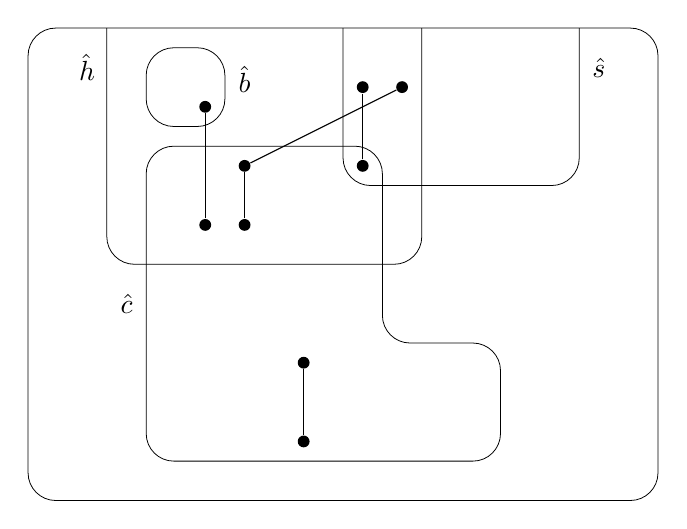
\begin{tikzpicture}[every node/.style={circle, fill=black, inner sep=0.5pt, minimum size=1.5mm}]
			]
			% \draw[help lines] (0,0) grid (8,6);
			\draw[rounded corners=10pt, line width=0.1mm] (0,0) rectangle (8,6);
			\draw[rounded corners=10pt, line width=0.1mm] (1,6) -- (1,3) -- (5,3) -- (5,6);
			\node[fill=none] (human) at (0.75,5.5) [] {$\hat{h}$};
			\draw[rounded corners=10pt, line width=0.1mm]
			(1.5,4.5) --
			(4.5,4.5) --
			(4.5,2) --
			(6,2) --
			(6,0.5) --
			(1.5,0.5) --
			cycle;
			\node[fill=none] (time) at (1.25,2.5) [] {$\hat{c}$};
			\draw[rounded corners=10pt, line width=0.1mm] (4,6) -- (4,4) -- (7,4) -- (7,6);
			\node[fill=none] (s) at (7.25, 5.5) [] {$\hat{s}$};

			\draw[rounded corners=10pt, line width=0.1mm] (1.5,5.75) rectangle (2.5,4.75);
			\node[fill=none] (billy) at (2.75,5.35) [] {$\hat{b}$};

			% minimal human
			% \draw[rounded corners=10pt, line width=0.2mm] (2,3) -- (2,4) -- (3,4) -- (3,3);
			% \node[fill=none] (minH) at (3.25,3.5) [] {$\underline{\hat{h}}$};
			\node (hb) at (2.25,3.5) [] {};
			\node (ht) at (2.25,5) [] {};
			\node (hr) at (2.75,3.5) [] {};
			\node (hrt) at (2.75,4.25) [] {};
			\draw (hr) -- (hrt);
			\draw (hb) -- (ht);

			% minimal soldier
			% \draw[rounded corners=10pt, line width=0.2mm] (5,5.25) -- (4.25,5.25) -- (4.25,4.25) -- (5,4.25);
			% \node[fill=none] (minS) at (5.25,5) [] {$\underline{\hat{s}}$};
			\node (sb) at (4.25, 4.25) [] {};
			\node (st) at (4.25, 5.25) [] {};
			\node (sr) at (4.75, 5.25) [] {};
			% \node (srr) at (5.5,5.625) [] {};
			\draw (sb) -- (st);
			\draw (sr) -- (hrt);

			% minimal time
			% \draw[rounded corners=10pt, line width=0.2mm] (3,0.5) -- (3,1.25) -- (4,1.25) -- (4,0.5);
			% \node[fill=none] (minC) at (4.25,1) [] {$\underline{\hat{c}}$};
			\node (cb) at (3.5,0.75) [] {};
			\node (ct) at (3.5,1.75) [] {};
			\draw (cb) -- (ct);
		\end{tikzpicture}
		\caption{A preferential model of $\Delta$}
		\label{figure:preferential-interpretation}
	\end{figure}
	\Cref{figure:preferential-interpretation} demonstrates one model of $\Delta$. It is relatively easy to verify that
	each statement (classical and defeasible) in $\Delta$ is satisfied by the preferential interpretation. As a means of providing
	some intuition for the preceding discussion, we remind the reader of \Cref{lemma:cut-cautious}, which says that ``If $\phi
		\twiddle \psi$, then the plausible consequences of $\phi \land \psi$ coincide with those of just $\phi$.'' As we have a
	model of $h \twiddle c$, the plausible consequences of $h$ and $h \land c$ should coincide. This Lemma becomes quite apparent
	when it is recognised that the two sets $\underline{\hat{h}}$ and $\underline{\widehat{h \land c}}$ are precisely the same
	sets.
	% The example further gives a good intution for why transitivity fails. Again, the interpretation is a model of $s \twiddle
	% h$ and $h \twiddle c$. For transitivity to hold,
\end{example}

Within the context of preferential models, there is another treatment of classical formulae which allows for the
discarding of \Cref{definition:state-satisfaction} and a single notion of what it means for a preferential
interpretation to be a model of a formula in $\Lang$. The idea is to translate the hard-constraints of classical formulae
to defeasible syntax.

\begin{lemma}
	\label{lemma:classical-to-defeasible}

	If $\phi$ is a classical formula in the language $\Lang$, then it can be expressed as the defeasible conditional $\neg
		\phi \twiddle \bot$. Then, any preferential interpretation $\pin$ is a model of $\phi$ if and only if it is a model of
	the defeasible conditional $\neg \phi \twiddle \bot$.
\end{lemma}

To explain the mechanics behind \Cref{lemma:classical-to-defeasible}, consider that a preferential interpretation $\pin$
being a model of the conditional $\neg \phi \twiddle \bot$ is equivalent to the $\neg \phi$-minimal states being a subset
of the states which satisfy $\bot$. Of course, $\bot$ represents logical falshood, and the set of states which satisfy
it is the emptyset. In turn, if $\pin$ is a model of $\neg \phi \twiddle \bot$, there can be no states which satisfy $\neg
	\phi$, which is equivalent to the condition that all states satisfy $\phi$. If $\phi$ is thought of as the proposition \say{All men are mortal},
then the defeasible counterpart reads as \say{If not all men are mortal, then it is normal to infer anything, including a contradiction}
\cite{kraus1990nonmonotonic,lehmann1992what}.

We assume this treatment of classical formulae from this point onwards, and consolidate the notation as $\pin \VDash \phi$
where $\phi \in \Lang$ is a defeasible conditional.

\textcolor{red}{maybe something about how without smoothness, we don't have CM}

\begin{theorem}[Soundness]
	\label{theorem:soundness-preferential}

	If $\Pin$ is a preferential interpretation and $\phi, \psi \in \Lang$, then $\pin$ defines the consequence relation $\twiddle
		_{\pin}$ given by the set $\{\phi \twiddle_{\pin}\psi \mid \pin \VDash \phi \twiddle \psi\}$, which satisfies \textit{Reflexivity},
	\textit{Left Logical Equivalence}, \textit{Right Weakening}, \textit{Or}, and \textit{Cautious Monotony} and is thus a
	preferential consequence relation.
\end{theorem}

\begin{theorem}[Completeness]
	\label{theorem:completeness-preferential}

	If $\twiddle_{P}$ is a preferential consequence relation, then there exists a preferential interpretation $W$ which induces
	the consequence relation $\twiddle_{W}$ such that $\twiddle_{P}$ is precisely $\twiddle_{W}$.
\end{theorem}

The decision to construct the preference relation on states which map to valuations, rather than valuations directly, may
seem arbitrary. Certainly, Shoham \cite{shohamSemanticApproach} makes no such distinction in his preferential logic.
However, Kraus, Lehmann, and Magidor \cite{kraus1990nonmonotonic} provide an example, apty described as ``en pessant''
by \cite{Bezzazi1997}, which shows that it is necessary in the setting of preferential consequence relations. The
example shows a preferential consequence relation generated by a preferential interpretation where the function mapping
states to valuations is not injective. It is then shown that there is no injective counterpart which gives rise to an equivalent
consequence relation.

\begin{lemma}
	\label{lemma:states-preferential}

	There exists a non-injective preferential interpretation $\pin$ which defines the consequence relation
	$\twiddle_{\pin}$ such that no injective preferential interpretation defines the same consequence relation.
\end{lemma}

\Cref{figure:duplicate-states-example} shows a portion of the preferential interpretation in
\Cref{example:preferential-interpretation}. The states $s_{1}$ and $s_{2}$ are duplicate states, specifically they both
map to the valuation $\{s,h,\overline{c}\}$. As before, this prefrential interpretation is a model of $s \twiddle h$ as
the set of minimal $s$-states, $\{s_{2},s_{3}\}$, is a subset of the $h$-states.

% Consider the more finely grained portion of the preferential interpretation in \Cref{figure:preferential-interpretation}.
% As before, the interpretation is a model of the conditional $s \twiddle h$. It is not, however, a model of $s \twiddle c$
% given that $s_{2}$, a duplicate state to $s_{1}$, is a minimal state satisfying $s$ which does not satisfy $c$.

\begin{figure}[H]
	\centering
	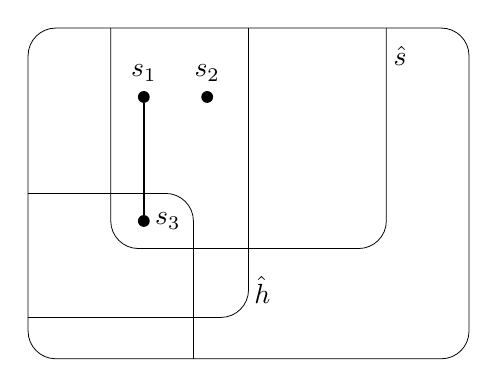
\begin{tikzpicture}[scale=0.7, every node/.style={circle, fill=black, inner sep=0.5pt, minimum size=1.5mm}]
		% \draw[help lines] (0,0) grid (8,6);
		\draw[rounded corners=10pt, line width=0.1mm] (0,0) rectangle (8,6);
		\draw[rounded corners=10pt, line width=0.1mm] (1.5, 6) -- (1.5,2) -- (6.5,2) -- (6.5,6);
		\draw[rounded corners=10pt, line width=0.1mm] (4,6) -- (4,0.75) -- (0,0.75);
		\draw[rounded corners=10pt, line width=0.1mm] (0,3) -- (3,3) -- (3,0);

		\node[fill=none] (h) at (4.25, 1.25) [] {$\hat{h}$};
		\node[fill=none] (s) at (6.75, 5.5) [] {$\hat{s}$};

		\node (1) at (2.1,4.75) [label=above:{$s_{1}$}] {};
		\node (2) at (3.25,4.75) [label=above:{$s_{2}$}] {};
		\node (3) at (2.1,2.5) [label=right:{$s_{3}$}] {};
		% \node (4) at (3.25,0.5) [label=right:{$s_{4}$}] {};
		\draw[line width=0.3mm] (1) -- (3);
		% \draw[line width=0.3mm] (2) -- (4);
	\end{tikzpicture}
	\caption{The \textit{en pessant} argument for allowing non-injective interpretations}
	\label{figure:duplicate-states-example}
\end{figure}

The interpretation is not a model of the conditional $s \twiddle c$, due to the counter-example of $s_{2}$ being a typical
soldier who does not experience chronological time. Should $s_{1}$ and $s_{2}$ be merged, the result would be an interpretation
which is a model of $s\twiddle c$; that is, a distinct consequence relation.

\subsection{Preferential Entailment}
\label{subsection:preferential-entailment}

Equipped with definitions for the class of preferential relations and a representation theorem that relates these to a
corresponding semantics in the form of preferential interpretations, it is appropriate to discuss the matter of \textit{preferential
	entailment}, or \textit{p-entailment}.

\begin{definition}
	\label{definition:p-entailment}

	A defeasible knowledge base $\Delta$ \textit{preferentially entails} a defeasible conditional $\phi \in \Lang$ if and only
	if $\phi$ is satisfied by every preferential model of $\Delta$, in this case we write $\Delta \dentails_{p}\phi$. The set
	of all defeasible conditionals that can be preferentially entailed from $\Delta$ is denoted by $\Cn{p}(\Delta)$ and is
	called the \textit{preferential closure} of $\Delta$.
\end{definition}

The definition provided for p-entailment is worryingly similar to the Tarskian idea of logical consequence, which was
described in \Cref{subsection:logical-consequence}. It is ``worrying'' in the sense that Tarskian consequence is monotonic,
and we are interested in non-monotonic entailment relations. Indeed, our fear is justified: If we consider the set of preferential
models of a defeasible knowledge base $\Delta$, then the set of conditionals they all agree on is exactly the
preferential closure, $\Cn{p}(\Delta)$. The addition of another conditional to our knowledge base, resulting in $\Delta \cup
	\{\phi \}$, only serves to reduce consideration to those models of $\Delta$ that also satisfy $\phi$. Within this restricted
set of models, the consensus on $\Cn{p}(\Delta )$ remains. Formally, we have:
\begin{align}
	\Delta \subseteq \Delta \cup \{\phi\} \quad \textit{implies}\quad \Cn{p}(\Delta) \subseteq \Cn{p}(\Delta \cup \{ \phi \})
\end{align}
which confirms our fear that p-entailment is monotonic.

There is room for some (justified) confusion here. After all, we have carefully avoided satisfying otherwise useful properties
because they imply monotonicity, only to end up with precisely that. To clarify this, we recognise that a system can
display non-monotonic behaviour in different areas. Indeed the entailment relation of system P---which reasons on the metalevel---is
monotonic, while the object level expresses non-monotonic behaviour, facilitating the expression of statements like \textit{Normally
	Humans experience chronological time}, \textit{Billy Pilgrim is a Human}, \textit{Billy Pilgrim experiences non-chronological
	time}.

There are arguments, in fact we make one in \textcolor{red}{chapter:defeasible-reasoning-in-fca}, which suggest that object
level non-monotonicity is sufficient.

% \begin{theorem}
% 	\label{theorem:preferential-compactness} If $\phi$ is a singular, and $\Delta$ a set of defeasible conditionals in
% 	$\Lang$, then the following equivalency holds:
% 	\begin{enumerate}
% 		\item The set $\Delta$ p-entails $\phi$; or, $\Delta \dentails_{p}\phi$

% 		\item There is a finite sequence consisting of the properties satisfied by preferential relations from $\Delta$ to $\phi$.
% 	\end{enumerate}
% \end{theorem}

% \begin{corollary}
% 	\label{corollary:monotonocity-preferential-entailment} The preferential closure $\Delta^{p}$ of a set $\Delta$ of defeasible
% 	conditionals is a preferential consequence relation, and therefore has a preferential model $\pin$ that satisfies
% 	exactly every statement in $\Delta^{p}$.
% \end{corollary}

% RE iT not being nmr We are willing to accept these credulous inferences precisely because they may be retracted we may withdraw
% previous inferences under learning new facts.

\subsection{Rational Consequence Relations}
\label{subsection:rational-consequence-relations}

System P provides a characterisation, in the form of its postulates, of a particular style of non-monotonic reasoning. There
are other kinds of reasoning, not valid in system P, for which there are good reasons think of as reasonable properties of
non-monotonic reasoning \cite{kraus1990nonmonotonic,lehmann1992what}.

\textit{Negation Rationality} suggests that our defeasible inferences should withstand piercing the veil of ignorance. Suppose
Alice is a university student, if she holds the belief that \textit{Normally, she will pass her exams}, then it would
not be reasonable for her to simultaneously think \textit{Normally, if she studies, she will not pass her exams} and also
\textit{Normally, if she does not study, she will not pass her exams}.
%
\begin{align}
	\inferLeft{Negation Rationality}{\phi \land \psi \ntwiddle \gamma, \quad \phi \land \neg \psi \ntwiddle \gamma}{\phi \ntwiddle \gamma}
\end{align}
Either Alice studies or she does not. If, in either case, she will not pass her exams, then it is difficult to comprehend
how it might be normal for her to pass her exams.

\textit{Disjunctive Rationality} says that a plausible inference made from a disjunction should be plausible from at
least one of the disjuncts.
\begin{align}
	\inferLeft{Disjunctive Rationality}{\phi \ntwiddle \gamma, \quad \psi \ntwiddle \gamma}{\phi \lor \psi \ntwiddle \gamma}
\end{align}

\textit{Rational monotony} is a much stronger form of restricted monotony than cautious monotony. Where cautious
monotony holds the position that we should only reason monotonically with the addition of new information that was
already expected given our beliefs, rational monotony suggests that we should reason monotonically with the addition of new
information if it is merely \textit{consistent} with existing beliefs; that is, we did not expect the negation of the
new information.
\begin{align}
	\inferLeft{Rational Monotony}{\phi \land \psi \ntwiddle \gamma, \quad \phi \ntwiddle \neg \psi }{\phi \ntwiddle \gamma}
\end{align}

Rational monotony can be equivalently stated as the following, which makes the intuition a bit clearer.
\begin{align}
	\inferLeft{Rational Monotony}{\phi \twiddle \psi, \quad \phi \ntwiddle \neg \gamma}{\phi \land \gamma \twiddle \psi}
\end{align}

At a university, it might be normal for students to graduate. At the same time, it would be too great a requirement to
suggest that it is normal for students to be exceptionally clever. It seems completely appropriate to maintain our belief
that it is normal for students, who are not exceptionally clever, to graduate.

Stalnaker \cite{Stalnaker1994,sep-logic-nonmonotonic-Stanford}, and separately Ginsberg \shortcite{GinsberCounterfactuals},
provide an argument against accepting rational monotony. The objection is that rational monotony commits us to make inferences
when the more reasonable position is to remain undecided. Paraphrasing, we are asked to consider three composers:
\textit{Verdi}, who is believed to be Italian, and \textit{Satie} and \textit{Bizet}, who are believed to be French. If it
were learned that Verdi and Bizet were compatriots, then it seems reasonable that the conclusion that either of them are
French or Italian is indeterminate. What is reasonable, however, is to maintain the belief that Satie is French.\footnote{We
	will use some syntax from predicate logic, this is merely an aid to make Stalnaker's example clearer.}
\begin{align}
	\texttt{Compatriots(Bizet, Verdi)}\twiddle \texttt{French(Satie)}
\end{align}
The argument proceeds by considering that Verdi and Satie may too be compatriots. Since Verdi's nationality is now
unknown, we are no longer equipped to reject the plausibility of the new compatriotship, and so
\begin{align}
	\texttt{Compatriots(Bizet, Verdi)}\ntwiddle \neg \texttt{Compatriots(Verdi,Satie)}
\end{align}
The two conditions of rational monotony have been met, and so the following inference should continue to hold
\begin{align}
	\texttt{Compatriots(Bizet, Verdi)}\land \texttt{Compatriots(Verdi,Satie)}\twiddle \texttt{French(Satie)}
\end{align}

The issue, as Stalnaker sees it, is that rational monotony forces the inference Satie is still French, and by their compatriotship,
so are Bizet and Verdi. The ``correct'' thing to do in this scenario is to remain uncertain about which nationality they
all share.

However, the result Stalnaker objects to is dependent his particular construction of this problem, rather than being intrinsic
to rational monotony. The second condition for rational monotony, that $\phi \ntwiddle \neg \gamma$, makes no
requirement about the syntactic structure of $\gamma$ outside of it being a formula in the language. In the example,
Stalnaker could just as easily have written
\begin{align}
	\texttt{Compatriots(Bizet,Verdi)}\ntwiddle \neg (\neg \texttt{Compatriots(Verdi,Satie))}
\end{align}
meaning that it is not expected that Verdi and Satie are compatriots, to which we can apply an instance of rational monotony,
from which we are not forced to believe that all three composers are French.
\begin{align}
	\texttt{Compatriots(Bizet, Verdi)}\land \neg(\texttt{Compatriots(Verdi,Satie))}\twiddle \texttt{French(Satie)}
\end{align}

There is another objection to rational monotony, which will be considered later on. For now, we accept it as a valid property
of non-monotonic reasoning, and thus introduce \textit{rational relations}.
%
\begin{definition}
	\label{definition:rational-relation}

	The consequence relation $\twiddle$ is a \emph{rational consequence relation} if and only if it satisfies the properties
	of \emph{Reflexivity}, \emph{Left Logical Equivalence}, \emph{Right Weakening}, \emph{And}, \emph{Or}, \emph{Cautious
		Monotony}, and \emph{Rational Monotony}.
\end{definition}

Quite evidently, they are a particular kind of preferential relation.

\subsubsection{Ranked Interpretations}
\label{subsubsection:ranked-interpretations}

From the knowledge that rational relations are a particular kind of preferential relation, it seems a reasonable jump to
think that the semantics we give to rational relations may be a particular kind of preferential interpretation. Before discussing
this jump, a useful exercise is to recognise how preferential interpretations may fail to satisfy rational monotony.

Consider the two preferential interpretations shown in \Cref{figure:two-preferential-models}, which model the scenario which
was discussed in the example near the end of the last subsection.

\begin{example}
	\label{example:university}

	Suppose that neither Alice nor Bob is a clever student. In spite of her status, Alice is considered by the preference
	relation to be a normal student, alongside Charlie. This situation is modelled in each of the preferential
	interpretations below.

	\begin{figure}[H]
		\centering
		\begin{minipage}{0.49\textwidth}
			\centering
			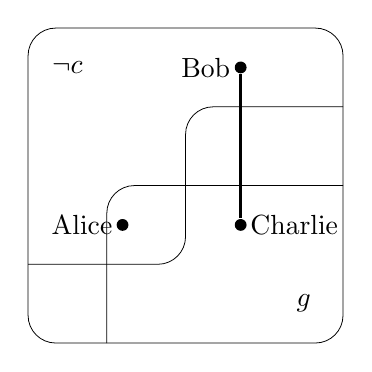
\begin{tikzpicture}[every node/.style={circle, fill=black, inner sep=0.5pt, minimum size=1.5mm}]
				% \draw[help lines] (0,0) grid (6,6);
				\draw[rounded corners=10pt, line width=0.1mm] (0,0) rectangle (4,4);
				\draw[rounded corners=10pt, line width=0.1mm] (0,1) -- (2,1) -- (2,3) -- (4,3);
				\draw[rounded corners=10pt, line width=0.1mm] (1,0) -- (1,2) -- (4,2);

				\node[fill=none] (clever) at (0.5,3.5) [] {$\neg c$};
				\node[fill=none] (graduated) at (3.5,0.5) [] {$g$};

				\node (bob) at (2.7,3.5) [label=left:{Bob}] {};
				\node (charlie) at (2.7,1.5) [label=right:{Charlie}] {};
				\draw[line width=0.3mm] (bob) -- (charlie);
				\node (alice) at (1.2,1.5) [label=left:{Alice}] {};
			\end{tikzpicture}
			\subcaption{Non-modular preference relation} \label{subfigure:not-rational}
		\end{minipage}
		\begin{minipage}{0.49\textwidth}
			\centering
			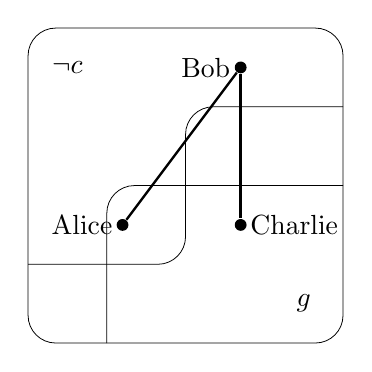
\begin{tikzpicture}[every node/.style={circle, fill=black, inner sep=0.5pt, minimum size=1.5mm}]
				\draw[rounded corners=10pt, line width=0.1mm] (0,0) rectangle (4,4);
				\draw[rounded corners=10pt, line width=0.1mm] (0,1) -- (2,1) -- (2,3) -- (4,3);
				\draw[rounded corners=10pt, line width=0.1mm] (1,0) -- (1,2) -- (4,2);

				\node[fill=none] (clever) at (0.5,3.5) [] {$\neg c$};
				\node[fill=none] (graduated) at (3.5,0.5) [] {$g$};

				\node (bob) at (2.7,3.5) [label=left:{Bob}] {};
				\node (charlie) at (2.7,1.5) [label=right:{Charlie}] {};
				\draw[line width=0.3mm] (bob) -- (charlie);
				\node (alice) at (1.2,1.5) [label=left:{Alice}] {};
				\draw[line width=0.3mm] (bob) -- (alice);
			\end{tikzpicture}
			\subcaption{Modular preference relation} \label{subfigure:rational}
		\end{minipage}
		\caption{ Two preferential models of the above scenario}
		\label{figure:two-preferential-models}
	\end{figure}

	We may verify that both are models of $\texttt{student}\twiddle \texttt{graduate}$, and neither are models of
	$\texttt{student}\twiddle \texttt{clever}$. By rational monotony, we should expect that
	$\texttt{student}\land \neg \texttt{clever}\twiddle \texttt{graduate}$ be satisfied, which is not the case in \Cref{subfigure:not-rational}.
\end{example}
%
Fortunately, the culprit is quite easy to spot. Bob, who is not under consideration in the context of normal students, appears
when we discuss normal students who are not clever. In isolation, this seems acceptable: if all the normal students were
also clever, then we would be fine accepting the appearance of a normal, non-clever student who was not a normal student.
However, we have explicitly ruled out this line of argument---by the second antecedent of rational monotony---as Alice
is a normal student who is also not clever.

In order to ensure rational monotony, it is required that the preference relation commit to Alice being preferred to Bob;
more generally, all normal students should be explicitly preferred to non-normal students. This notion is formalised by
the following property called \textit{modualarity}:

\begin{definition}
	\label{definition:modular-order} \index{partial-order! modular}

	A partial order $\prec$ on the set $X$ is \emph{modular} if and only if for any incomparable $x,y \in X$ when $z \prec
		x$ then also $z \prec y$.
\end{definition}

One perspective on \textit{modular} partial orders is that they partition the set of states into equivalence classes of preference,
so that all states in the same class are incomparable to one another \cite{GinsberCounterfactuals}. Then, if the
preference relation is defined as the equivalence relation itself, such that one state is preferred to another if the class
it belongs to is preferred to the other's, we get a modular order.

\begin{definition}
	\label{definition:ranked-interpretation}

	A \emph{ranked interpretation} is a preferential interpretation $\Pin$ where the preference relation $\prec$ is \emph{modular}.
\end{definition}

A somewhat superficial result of ranked interpretations is that they admit a new representation as a stratified equivalence
relation, depicted in \Cref{figure:ranked-interpretation-representation}. Each strata, or \textit{rank}, has an
associated ordinal.

\begin{lemma}
	\label{lemma:modular-ranking-function}

	If $\prec$ is a modular partial order on $X$ then there is a \emph{ranking function} $\mathsf{r}\colon X \to \Omega$,
	with $\Omega$ being a totally ordered set for which the strict order is denoted $<$, such that if $x \prec y$ then $\mathsf{r}
		(x) < \mathsf{r}(y)$ for any $x,y \in X$.
\end{lemma}

\begin{figure}[H]
	\centering
	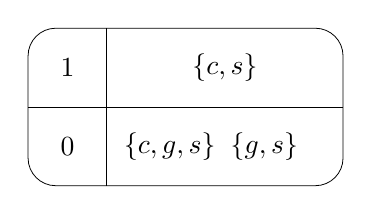
\begin{tikzpicture}[every node/.style={circle, fill=black, inner sep=0.5pt, minimum size=1.5mm}]
		\draw[rounded corners=10pt, line width=0.1mm] (0,2) rectangle (4,0);
		\draw[rounded corners=10pt, line width=0.1mm] (0,1) -- (4,1);
		\node[fill=none] (0) at (0.5,0.5) [] {$0$};
		\node[fill=none] (1) at (0.5,1.5) [] {$1$};
		\draw (1,0) -- (1,2);
		\node[fill=none] (alice) at (1.8,0.5) [] {$\{c,g,s\}$};
		\node[fill=none] (charlie) at (3,0.5) [] {$\{g,s\}$};
		\node[fill=none] (bob) at (2.5,1.5) [] {$\{c,s\}$};
	\end{tikzpicture}
	\caption{A depiction of a ranked interpretation}
	\label{figure:ranked-interpretation-representation}
\end{figure}

A second, less superficial, departure is that \Cref{lemma:states-preferential} does not hold in the context of ranked
interpretations and rational consequence relations. This follows directly from modularity, as the en pessant style
arguments, discussed earlier, are avoided by modularity. This allows the elements which populate the ranks of a ranked interpretation
to be valuations directly, rather than states.

\begin{definition}
	\label{definition:ranked-interpretation-real}

	A \emph{ranked interpretation} is a function $\mathsf{r}\colon \mathcal{U}\to \mathbb{N}$
\end{definition}

\textcolor{red}{Talk about smoothness with ranked models}

\subsection{Ranked Entailment}
\label{subsection:ranked-entailment}

\section{Rational Closure}
\label{section:rational-closure}
